
\documentclass[11pt,english]{beamer}
%\documentclass[11pt]{beamer}
\usepackage{mathptmx}
\renewcommand{\sfdefault}{lmss}
\renewcommand{\familydefault}{\sfdefault}
\usepackage[T1]{fontenc}
\usepackage[latin9]{inputenc}
\usepackage{amsmath}
\usepackage{amssymb}
\usepackage{graphicx}
\PassOptionsToPackage{normalem}{ulem}
\usepackage{ulem}
\usepackage{caption}
\captionsetup{labelformat=empty}
\usepackage{bbm}
\usepackage{upgreek}
\usepackage{graphicx}
\setbeamertemplate{section in toc}[sections numbered]
\makeatletter
\usepackage{caption} 
\captionsetup[table]{skip=10pt}
%%%%%%%%%%%%%%%%%%%%%%%%%%%%%% Textclass specific LaTeX commands.
 % this default might be overridden by plain title style
 \newcommand\makebeamertitle{\frame{\maketitle}}%
 % (ERT) argument for the TOC
 \AtBeginDocument{%
   \let\origtableofcontents=\tableofcontents
   \def\tableofcontents{\@ifnextchar[{\origtableofcontents}{\gobbletableofcontents}}
   \def\gobbletableofcontents#1{\origtableofcontents}
 }


\setbeamersize{text margin left= .8em,text margin right=1em} 
\newenvironment{wideitemize}{\itemize\addtolength{\itemsep}{10pt}}{\enditemize}
\newenvironment{wideitemizeshort}{\itemize}{\enditemize}

%%%%%%%%%%%%%%%%%%%%%%%%%%%%%% User specified LaTeX commands.
%\documentclass[presentation]{beamer}


\def\Tiny{\fontsize{7pt}{8pt}\selectfont}
\def\Normal{\fontsize{8pt}{10pt}\selectfont}

\usetheme{Madrid}
\usecolortheme{lily}
%\setbeamercovered{transparent}
\useinnertheme{rounded}


\setbeamertemplate{footline}{\hfill\Normal{\insertframenumber/\inserttotalframenumber}}
%\setbeamertemplate{footline}{}

\setbeamertemplate{navigation symbols}{}

\newenvironment{changemargin}[2]{%
\begin{list}{}{%
\setlength{\topsep}{0pt}%
\setlength{\leftmargin}{#1}%
\setlength{\rightmargin}{#2}%
\setlength{\listparindent}{\parindent}%
\setlength{\itemindent}{\parindent}%
\setlength{\parsep}{\parskip}% 
}%
\item[]}{\end{list}}

\setbeamertemplate{footline}{\hfill\insertframenumber/\inserttotalframenumber}
\setbeamertemplate{navigation symbols}{}

%\usepackage{times}  % fonts are up to you
\usepackage{graphicx}
%\usepackage{graphics}
\usepackage{epsfig}
\usepackage{bm}
\usepackage{epsf}
\usepackage{float}
\usepackage[final]{pdfpages}
\usepackage{multirow}
\usepackage{colortbl}
\usepackage{xkeyval}
%\usepackage{sgame}
%\usepackage{pst-node}
\usepackage{listings}
\usepackage{ifthen}
%\usepackage{hyperref}
\usepackage{tikz}

%\usepackage{times}  % fonts are up to you
%\usepackage{graphicx}
%\usepackage{graphics}
\usepackage{epsfig,bm,epsf,float}
\usepackage[final]{pdfpages}
\usepackage{xcolor,multirow,colortbl}
\usepackage{xkeyval}
\usepackage{verbatim}
%\usepackage{sgame}
%\usepackage{pst-node}
\usepackage{listings}
%\usepackage{handoutWithNotes}
%\pgfpagesuselayout{3 on 1 with notes}[letterpaper,border shrink=5mm]
%\pgfpagesuselayout{2 on 1 with notes landscape}[letterpaper,border shrink=5mm]
\usepackage{setspace}
\usepackage{ragged2e}

\setbeamersize{text margin left=1em,text margin right=1em} % CambridgeUS spacing if you use default instead


%\pdfmapfile{+sansmathaccent.map}

% Table formatting
\usepackage{booktabs}


% Decimal align
\usepackage{dcolumn}
\newcolumntype{d}[0]{D{.}{.}{5}}

\newcommand\independent{\protect\mathpalette{\protect\independenT}{\perp}}
\def\independenT#1#2{\mathrel{\rlap{$#1#2$}\mkern2mu{#1#2}}}

\global\long\def\expec#1{\mathbb{E}\left[#1\right]}
\global\long\def\var#1{\mathrm{Var}\left[#1\right]}
\global\long\def\cov#1{\mathrm{Cov}\left[#1\right]}
\global\long\def\prob#1{\mathrm{Prob}\left[#1\right]}
\global\long\def\one{\mathbf{1}}
\global\long\def\diag{\operatorname{diag}}
\global\long\def\expe#1#2{\mathbb{E}_{#1}\left[#2\right]}
\DeclareMathOperator*{\plim}{\text{plim}}

%\usefonttheme[onlymath]{serif}

\usepackage{appendixnumberbeamer}
\renewcommand{\thefootnote}{}

\setbeamertemplate{footline}
        {
      \leavevmode%
   %   \hbox{%
%      \begin{beamercolorbox}[wd=\paperwidth,ht=2.25ex,dp=1ex,right]{date in head/foot}%
        %\usebeamerfont{date in head/foot}\insertshortdate{}\hspace*{2em}%
\hfill
    %turning the next line into a comment, erases the frame numbers
        \insertframenumber{}\hspace*{2ex}\vspace{1ex}

  %    \end{beamercolorbox}}%
}

\definecolor{blue}{RGB}{0, 0, 210}
\definecolor{red}{RGB}{170, 0, 0}

\makeatother

\usepackage[english]{babel}

%\mode<handout>{
  %\setbeamercolor{background canvas}{bg=black!5}
  %\usepackage{pgfpages}
  %\pgfpagesuselayout{2 on 1}[a4paper,border shrink=5mm]
 %\pgfpagesuselayout{4 on 1}[a4paper,border shrink=5mm,landscape]
%}
%\newcommand{\opause}{\pause{}} 

\usepackage{tikz}
\newcommand*\circled[1]{\tikz[baseline=(char.base)]{             \node[circle,ball color=structure.fg, shade,   color=white,inner sep=1.2pt] (char) {\tiny #1};}} 

\makeatletter
\let\save@measuring@true\measuring@true
\def\measuring@true{%
  \save@measuring@true
  \def\beamer@sortzero##1{\beamer@ifnextcharospec{\beamer@sortzeroread{##1}}{}}%
  \def\beamer@sortzeroread##1<##2>{}%
  \def\beamer@finalnospec{}%
}
\makeatother

\begin{document}

%% Title slide
\begin{frame}[noframenumbering]{}
\vspace{0.5cm}
\title[]{Day 2: On Weights and Clusters}
\author{Peter Hull}
\date{Design-Based Regression Inference \\Spring 2024} 
\titlepage {\small{}\ }\thispagestyle{empty} \vspace{-30pt}

\end{frame}
 

\begin{frame}{Outline}

1. Heterogeneous Treatment Effects
\vspace{0.8cm}

2. Clustered Standard Errors

\end{frame}

\begin{frame}{Whose Treatment Effect is it Anyway?}
\begin{itemize}
\item On Monday we contrasted design vs. outcome-model strategies in a constant-effect world (i.e. with a causal model of $y_i=\beta x_i+\varepsilon_i$)\smallskip
\begin{itemize}
\item Of course the real world is messier: more realistic is $y_i=\beta_i x_i+\varepsilon_i$ \\ (or more complicated forms of effect heterogeneity) \smallskip\pause{}
\item Can think about what the regression/IV estimand equals in such models
\end{itemize}\bigskip\pause{}
\item Today we'll see another difference: how design-based vs. model-based regression/IV weigh together heterogeneous effects\smallskip
\begin{itemize}
\item Bottom line: design avoids recent concerns over ``negative weights''...\smallskip\pause{}
\item ... at least as long as you don't have multiple treatments! 
\end{itemize}
\end{itemize}
\end{frame}

\begin{frame}{Why So Negative?}

\begin{itemize}
\item A recent TWFE literature (e.g. de Chaisemartin and D'Haultfoeuille '20; Goodman-Bacon '21; Borusyak et al. '23) shows that some regressions identify $\beta = E[\psi_i \beta_i]/E[\psi_i]$ for possibly negative $\psi_i$\smallskip\pause{}
\begin{itemize}
\item We'll term these $\psi_i$ ``ex-post'' weights, for reasons you'll see shortly\bigskip\pause{}
\end{itemize}
\item Why is this a concern? The possibility of \emph{sign reversals}:\smallskip
\begin{itemize}
\item Even if all $\beta_i$ are positive, $\beta$ could wind up negative (or vice versa) if $\psi_i$ and $\beta_i$ are correlated \smallskip
\item The literature proposes alternative specifications/procedures that avoid negative weighting or allow for custom-built weights
\end{itemize}\bigskip\pause{}
\item It turns out that such $\psi_i$ also arise in design-based specifications, and they can also be negative\smallskip
\begin{itemize}
\item But sign reversals are impossible in design-based specs: then we also have $\beta=E[\phi_i\beta_i]/E[\phi_i]$ for ``ex-ante'' $\phi_i$ which are always non-negative
\end{itemize}
\end{itemize}

\end{frame}

\begin{frame}{Simple Setup}
\begin{itemize}
\item Suppose a researcher estimates by OLS:
\begin{align*}
y_i=\beta x_i + w_i^\prime \gamma + e_i
\end{align*}
for some outcome $y_i$, treatment $x_i$, and vector of controls $w_i$\bigskip\pause{}
\item To interpret $\beta$, we consider a linear-effect causal model:
\begin{align*}
y_i = \beta_i x_i + \varepsilon_i
\end{align*}
with heterogeneous effects $\beta_i$ and untreated potential outcomes $\varepsilon_i$\smallskip
\begin{itemize}
\item Note: for binary $x_i$ this is the more familiar $y_i=(y_i(1)-y_i(0))x_i + y_i(0)$
\end{itemize}\medskip\pause{}
\item Assume appropriate asymptotics for OLS to consistently estimate:
\begin{align*}
\beta = \frac{E[\tilde{x}_i y_i]}{E[\tilde{x}_i^2]}=\frac{E[\tilde{x}_i x_i\beta]+E[\tilde{x}_i\varepsilon_i]}{E[\tilde{x}_i^2]}
\end{align*}
where $\tilde{x}_i$ are residuals from the population regression of $x_i$ on $w_i$
\end{itemize}
\end{frame}

\begin{frame}{Two Paths to Avoiding Omitted Variables Bias}

\begin{itemize}
\item $E[\tilde{x}_i\varepsilon_i]=0$ under either one of two assumptions:
\bigskip\pause{}

ASSUMPTION 1: $E[\varepsilon_i\mid x_i,w_i]=w_i^\prime\gamma$
\smallskip
\begin{itemize}
\item Untreated potential outcomes are linear in controls, given treatment\smallskip
\item E.g. parallel trends, where $i$ indexes unit-period pairs in a panel and $w_i$ includes unit and time dummies
\end{itemize}
\bigskip\pause{}

ASSUMPTION 2: $E[x_i\mid \varepsilon_i,\beta_i,w_i]=w_i^\prime\lambda$
\smallskip
\begin{itemize}
\item Treatment is conditionally mean-independent
of potential outcomes, with a linear \emph{expected
treatment} $E[x_i\mid w_i]$ (e.g. the propensity score)\smallskip
\item E.g. a stratified experiment, where $x_i$ is randomly assigned within strata dummied out in $w_i$ \smallskip
\item Note we're conditioning on \emph{both} $\varepsilon_i$ and $\beta_i$, ruling out ``selection on gains'' (will relax with IV version soon)
\end{itemize}
\bigskip\pause{}

\item The second assumption yields a design-based OLS specification\smallskip
\begin{itemize}
\item Stronger (sufficient) condition: $x_i\mid (\varepsilon_i,\beta_i,w_i)\stackrel{iid}{\sim} G(w_i)$
\end{itemize}
\end{itemize}

\end{frame}

\begin{frame}{Ex-Post Weights}

\begin{itemize}
\item Since $E[\tilde{x}_i\varepsilon_i]=0$, the OLS estimand has an average-effect representation under either assumption:
\begin{equation*}
\beta= \frac{E[\psi_i\beta_i]}{E[\psi_i]},\quad\quad \psi_i=\tilde{x}_ix_i
\end{equation*}
\pause{}

\item But the ex-post weights $\psi_i$ are generally non-convex: $E[\tilde{x}_i]=0$, so \\ $\tilde{x}_i$ must take on both positive and negative values\smallskip \pause{}
\begin{itemize}
\item E.g. if $x_i>0$ then $i$ with low values of $x_i$ (the effective control group) will always receive negative ex-post weight\smallskip\pause{}
\item This can lead to sign reversals: e.g. $\beta<0$, despite $\beta_i>0$
\end{itemize}
\bigskip\pause{}

\item The ex-post weights are the end of the story for $\beta$ under Assumption 1. But in design-based specifications we can take one more step\smallskip
\begin{itemize}
\item In experiments, who is in the effective control group is \emph{random}. Before treatment is drawn, everyone expects the same weight!
\end{itemize}
\end{itemize}

\end{frame}

\begin{frame}{Ex-Ante Weights}

\begin{itemize}
\item Using the law of iterated expectations, we can also write:
\begin{equation*}
\beta= \frac{E[E[\psi_i\mid w_i,\beta_i]\beta_i]}{E[E[\psi_i\mid w_i,\beta_i]]}\equiv \frac{E[\phi_i\beta_i]}{E[\phi_i]}
\end{equation*}
for ex-ante weights $\phi_i = E[\tilde{x}_ix_i\mid w_i,\beta_i]$
\pause{}\smallskip
\begin{itemize}
\item Under Assumption 1, this need not help: i.e. if treatment is deterministic in the unit/time FE in $w_i$, then $\phi_i=\psi_i$\pause{}
\end{itemize}\bigskip 

\item But under Assumption 2, $\phi_i=Var(x_i\mid w_i,\beta_i)$ which is non-negative!\smallskip\pause{}
\begin{itemize}
\item $E[\tilde{x}_ix_i\mid w_i,\beta_i]=E[\tilde{x}_i^2\mid w_i,\beta_i]+E[\tilde{x}_i\mid w_i,\beta_i]w_i^\prime\lambda=Var(x_i\mid w_i,\beta_i)+0$
\end{itemize}\bigskip\pause{}
\item Hence: sign reversals cannot occur in design-based OLS specifications
\end{itemize}
\end{frame}
\begin{frame}{Interpretation}
\begin{itemize}
\item Even if we formulate a design-based regression in terms of constant effects, the estimand is still reasonable under heterogeneous effects\smallskip
\begin{itemize}
\item Not necessarily true for outcome models (makes sense: we were just modeling $\varepsilon_i$! But additional models on $\beta_i$ need not help)
\end{itemize}\medskip\pause{}
\item With the stronger design assumption of $x_i\mid (\varepsilon_i,\beta_i,w_i)\stackrel{iid}{\sim} G(w_i)$, the ex ante weights become identified: $\phi_i=Var(x_i\mid w_i,\beta_i)=Var(x_i\mid w_i)$\smallskip
\begin{itemize}
\item C.f. earlier results in Angrist (1998), Angrist and Krueger (1999), etc\smallskip\pause{}
\item Could inverse-weight by $\widehat{Var}(x_i\mid w_i)$ to estimate unweighted $E[\beta_i]$
\end{itemize}\medskip\pause{}
\item Of course, the $\phi_i$-weighted estimand may not be most of interest!\smallskip
\begin{itemize}
\item If $Cov(\phi_i,\beta_i)\approx 0$, we'll still get something close to $E[\beta_i]$\smallskip
\item Otherwise, $\phi_i$-weighting has desirable efficiency properties (Goldsmith-Pinkham et al. 2024)\smallskip
\item Large class of alternative propensity-score-based estimators for other estimands under the stronger design assumption
\end{itemize}
\end{itemize}
\end{frame}

\begin{frame}{General Setting}
\begin{itemize}
\item Borusyak and Hull (2024) extend ex ante / ex post weights to:\smallskip
\begin{enumerate}
\item A more general causal model: potential outcomes $y_i(x)$ and $y_i=y_i(x_i)$\smallskip
\item IV: design-based assumption is then $E[z_i\mid y_i(\cdot),w_i]=w_i^\prime\lambda$
\end{enumerate}\bigskip\pause{}
\item For convex ex-ante weights in IV we require first-stage \emph{monotonicity}: that $x_i$ is non-decreasing in $z_i$ for all units regardless of $y_i(\cdot)$ \smallskip
\begin{itemize}
\item C.f. earlier results in Imbens and Angrist ('94, '95), Angrist et al. ('00)\smallskip\pause{}
\item Ex post weights are still potentially non-convex under monotonicity 
\end{itemize}\bigskip\pause{}
\item Framework is general, allowing for ``formula'' IVs (e.g. shift-share)\smallskip
\begin{itemize}
\item We'll see more about this in Friday's class
\end{itemize}
\end{itemize}
\end{frame}

\begin{frame}{Multiple Treatments: Contamination Bias}
\begin{itemize}
\item Goldsmith-Pinkham et al. (2024) generalize things in a different direction: hetFX weighting for regressions w/multiple treatments\smallskip
\begin{itemize}
\item Unfortunately the picture is a bit less rosy for design here
\end{itemize}\bigskip\pause{}
\item The coefficient on treatment $j$ estimates the sum of two terms:\smallskip
\begin{enumerate}
\item A weighted average of treatment $j$'s effects, with convex weights in design-based specifications $\checkmark$\smallskip\pause{}
\item A non-convex combination of effects from other treatments $k$ (``contamination bias'') $\text{\sffamily X}$
\end{enumerate}\bigskip\pause{}
\item They derive alternative estimators which avoid contamination bias while maintaining the nice efficiency properties of OLS weighting\smallskip
\begin{itemize}
\item Ultimately, becomes an empirical question of how important bias is
\end{itemize}
\end{itemize}
\end{frame}

\begin{frame}{Example: Project STAR}

\begin{itemize}
\item Krueger (1999) studies the STAR RCT, which randomized 12k students in 80 public elementary schools in Tennessee to one of 3 classroom types:\smallskip
\begin{enumerate}
\item Regular-sized (20-25 students) -- Control\smallskip
\item Small (13-17 students) -- Treatment 1\smallskip
\item Regular-sized with a teaching aide -- Treatment 2
\end{enumerate}\bigskip\pause{}

\item Kids were randomized within schools, so the propensity of assignment to each treatment varied by school\smallskip
\begin{itemize}
\item Krueger thus estimates: $TestScore_i= \alpha_{school(i)}+\beta_1 D_{i1} + \beta_2 D_{i2} +\varepsilon_i$
\end{itemize}\bigskip\pause{}

\item We find significant \emph{potential} for contamination bias: lots of treatment effect heterogeneity and variation in contamination weights\smallskip
\begin{itemize}
\item But actual contamination bias is minimal: $Corr(effects,weights)\approx 0$
\end{itemize}
\end{itemize}

\end{frame}

\begin{frame}{Project STAR, Revisited}

\begin{center}
	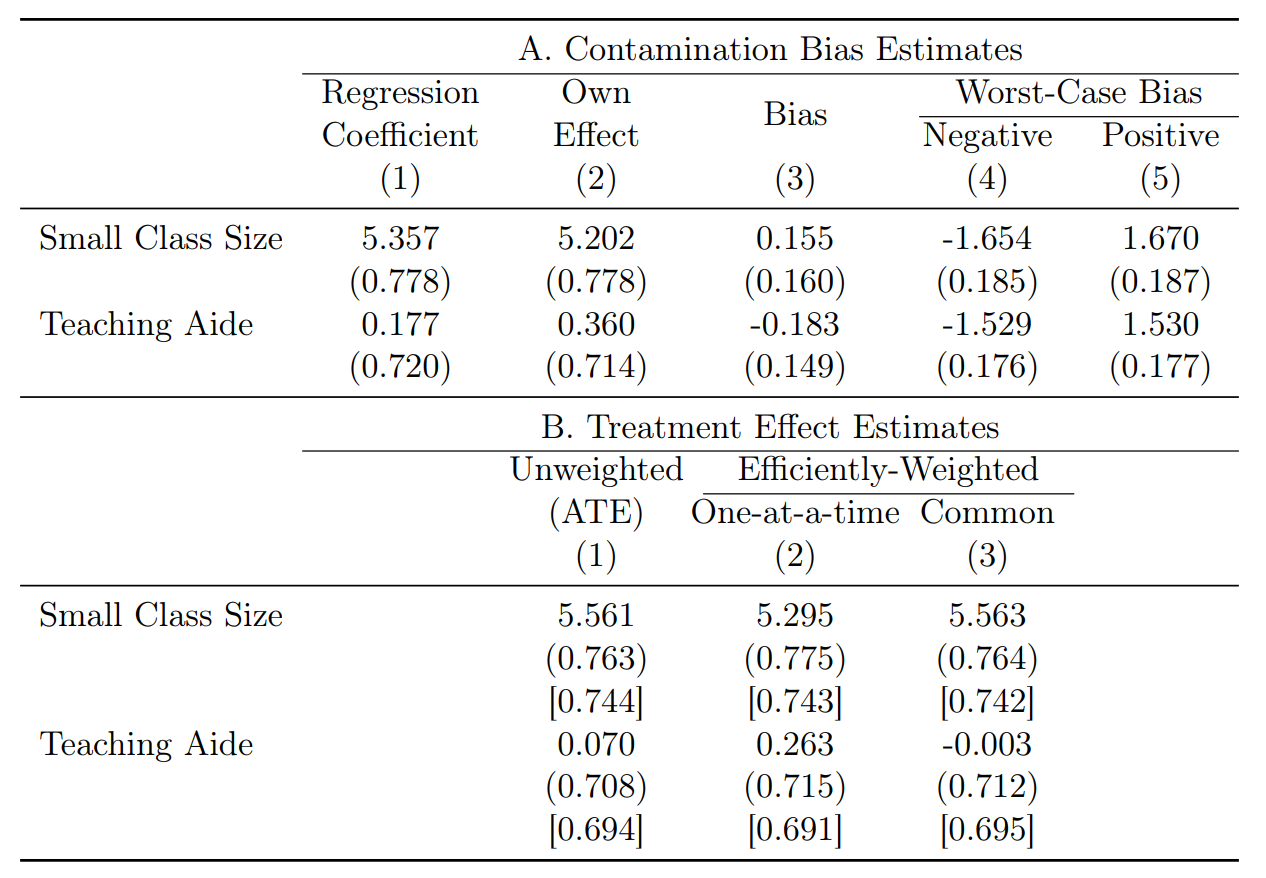
\includegraphics[width=0.9\textwidth]{figures/STAR_CB.png}
\end{center}

\end{frame}

\begin{frame}{STAR Regression Weights vs. Treatment Effects}
\vspace{0.1cm}
\begin{center}
	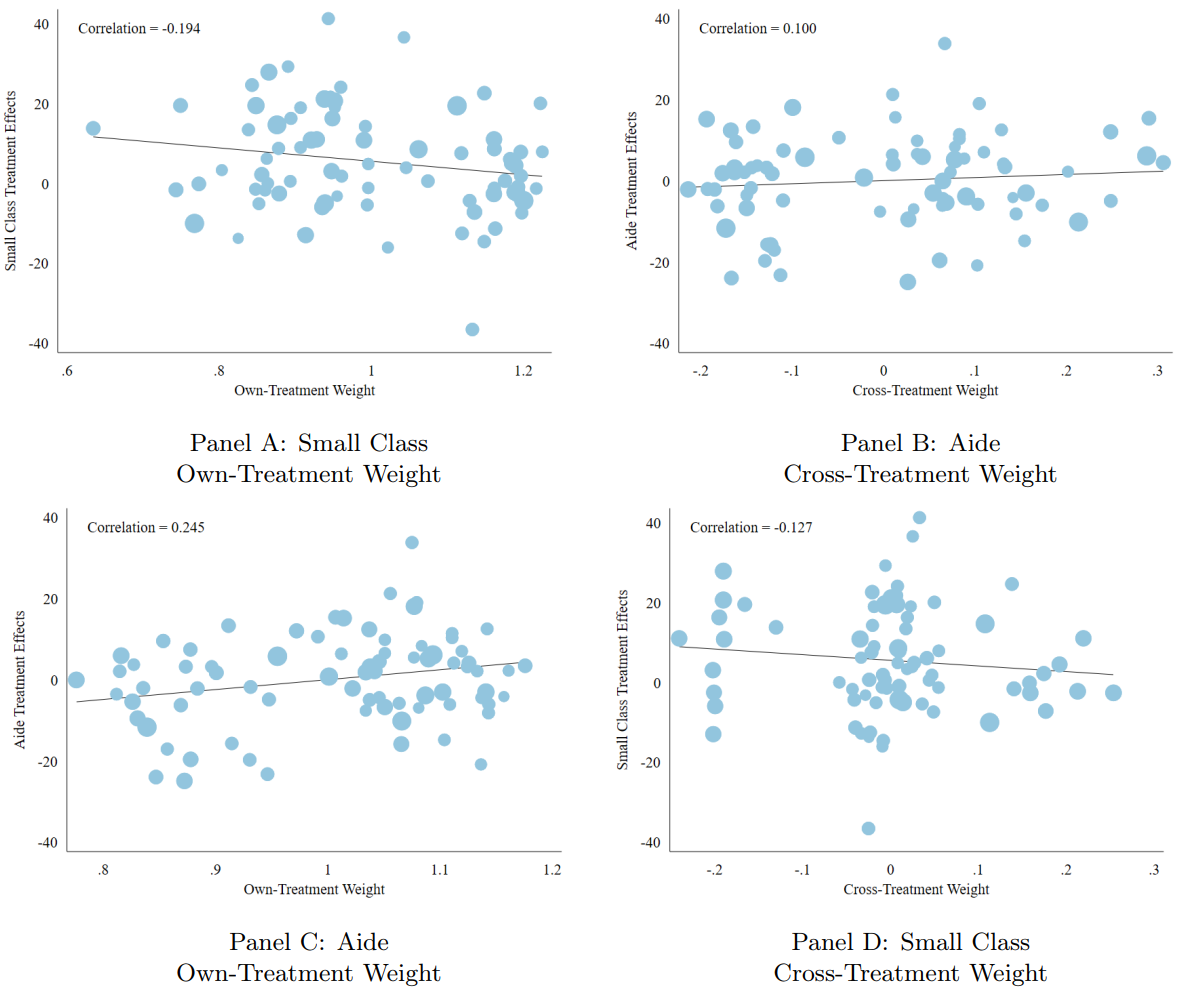
\includegraphics[width=0.82\textwidth]{figures/STAR_Scatter.png}
\end{center}

\end{frame}

\begin{frame}{Outline}

\textcolor{red!75!green!50!blue!25!gray}{1. Heterogeneous Treatment Effects}$\checkmark$
\vspace{0.8cm}

2. Clustered Standard Errors

\end{frame}

\begin{frame}{OLS Asymptotics: Review}

\begin{itemize}
\item Where do SEs come from? OLS $\hat\beta=(\mathbf{X}^\prime\mathbf{X})^{-1}\mathbf{X}^\prime\mathbf{Y}$ can be rewritten:
\begin{align*}
\sqrt{N}(\hat\beta - \beta) = \left(\frac{\mathbf{X}^\prime\mathbf{X}}{N}\right)^{-1} \left(\frac{\mathbf{X}^\prime\boldsymbol\varepsilon}{\sqrt{N}}\right)
\end{align*}
where $\mathbf{Y}=\mathbf{X}\beta + \boldsymbol{\varepsilon}$ stacks observations of the population regression \smallskip\pause{}
\begin{itemize}
\item Under rather mild conditions (a LLN), $\frac{\mathbf{X}^\prime\mathbf{X}}{N}\xrightarrow{p}E\left[\frac{1}{N}\sum_i X_iX_i^\prime\right]$\smallskip\pause{}
\item W/slightly stronger conditions (a CLT), $\frac{\mathbf{X}^\prime\boldsymbol\varepsilon}{\sqrt{N}}\Rightarrow \mathrm{N}(0,Var(\frac{1}{\sqrt{N}}\sum_i X_i\varepsilon_i))$
\end{itemize}\medskip\pause{}
\item This gives our general asymptotic approximation for OLS: $\hat\beta\approx\beta^*$ for
\end{itemize}
\begin{align*}
\beta^* \sim \mathrm{N}(\beta,\frac{V}{N}),\hspace{0.2cm} V=E\left[\frac{1}{N}\sum_i X_iX_i^\prime\right]^{-1} Var\left(\frac{1}{\sqrt{N}}\sum_i X_i\varepsilon_i\right) E\left[\frac{1}{N}\sum_i X_iX_i^\prime\right]^{-1}
\end{align*}\pause{}
\begin{itemize}
\item SEs come from $\hat{V}=\left(\frac{1}{N}\sum_i X_iX_i^\prime\right)^{-1} \widehat{Var}\left(\frac{1}{\sqrt{N}}\sum_i X_i\varepsilon_i\right) \left(\frac{1}{N}\sum_i X_iX_i^\prime\right)^{-1}$
\end{itemize}
\end{frame}

\begin{frame}{Getting to the Meat of the ``Sandwich Estimator,'' $\hat{V}$}

\begin{itemize}
\item Key q: how do we form the variance estimate $\widehat{Var}\left(\frac{1}{\sqrt{N}}\sum_i X_i\varepsilon_i\right)$?\bigskip\pause{}

\item In \emph{iid} data, we know $Var\left(\frac{1}{\sqrt{N}}\sum_i X_i\varepsilon_i\right)=\pause{}\frac{1}{N}\sum_i Var(X_i\varepsilon_i)=\pause{}E[X_iX_i^\prime\varepsilon_i^2]$\smallskip
\begin{itemize}\pause{}
\item This suggests $\widehat{Var}\left(\frac{1}{\sqrt{N}}\sum_i X_i\varepsilon_i^2\right)=\frac{1}{N}\sum_iX_iX_i^\prime\hat\varepsilon_i^2$, which leads to our usual heteroskedasticity-robust estimator
\end{itemize}\bigskip\pause{}

\item The motivation for alternative estimators comes from the possibility that $X_i\varepsilon_i$ and $X_j\varepsilon_j$ may be correlated for $i\neq j$\smallskip
\begin{itemize}
\item Generally,  $Var\left(\frac{1}{\sqrt{N}}\sum_i X_i\varepsilon_i\right)=\frac{1}{N}\sum _i Var(X_i\varepsilon_i)+2\sum_{i,j\neq i}Cov(X_i\varepsilon_i,X_j\varepsilon_j)$\smallskip\pause{}
\item But we can't allow for arbitrary cross-sectional correlations, since then we couldn't guarantee $\frac{1}{\sqrt{N}}\sum_i X_i\varepsilon_i$ converges ... \smallskip\pause{}
\item We need to zero out some covariances to make progress
\end{itemize}
\end{itemize}
\end{frame}

\begin{frame}{Cluster-Robust Estimators}
\begin{itemize}
\item Suppose we can partition observations into clusters, $c(i)\in{1,\dots,C}$\smallskip
\begin{itemize}
\item To ease notation, suppose equal sizes: $|i:c(i)=c|=N/C\equiv T$\smallskip\pause{}
\item With $N=CT$, OLS can be rewritten: $\sqrt{N}(\hat\beta - \beta) = \left(\frac{\mathbf{X}^\prime\mathbf{X}}{N}\right)^{-1}\cdot \left(\frac{\mathbf{X}^\prime\boldsymbol\varepsilon}{\sqrt{CT}}\right)$
\end{itemize}\medskip\pause{}

\item Define $Q_c=\frac{1}{\sqrt T}\sum_{i:c(i)=c}X_i\varepsilon_i$ and note that $\frac{\mathbf{X}^\prime\boldsymbol\varepsilon}{\sqrt{CT}}=\frac{1}{\sqrt{C}}\sum_c Q_c$\smallskip\pause{}
\begin{itemize}
\item If the $Q_c$ clusters are \emph{iid}, a CLT applies: $\frac{1}{\sqrt{C}}\sum_c Q_c\Rightarrow \mathrm{N}(0,Var(Q_c))$\smallskip
\item E.g. in a balanced panel, could have \emph{iid} series $(X_{c1}\varepsilon_{c1}\dots,X_{cT}\varepsilon_{cT})$
\end{itemize}\medskip\pause{}

\item This gives us a new ``clustered'' variance estimate to plug into $\hat{V}$:
\begin{align*}
\widehat{Var}\left(\frac{1}{\sqrt{N}}\sum_i X_i\varepsilon_i\right)=\frac{1}{C}\sum_c \hat{Q}_c^2,\text{ for }\hat{Q}=\frac{1}{\sqrt{T}}\sum_{i:c(i)=c}X_i\hat\varepsilon_i
\end{align*}\pause{}

\item This is what's going on under the hood when you ``\emph{, cluster(c)}''!
\end{itemize}
\end{frame}

\begin{frame}{Easy, Right?}

\begin{center}
	
\includegraphics[width=0.6\textwidth]{figures/khoa_cluster.jpg}
\end{center}
\hspace{\fill}Source: Khoa Vu (of course)
\end{frame}

\begin{frame}{Design Can Help!} 
\begin{itemize}
\item At an (unhelpfully) high level, the previous results tell us when to cluster $i$ and $j$ together: when we think $Cov(X_i\varepsilon_i,X_j\varepsilon_j)\neq 0$\bigskip\pause{}
\item With design this may not be too hard to figure out:\smallskip
\begin{itemize}
\item Suppose $(X_1,\dots,X_N)
\mid (\varepsilon_1,\dots,\varepsilon_N)$ is mean-zero with $X_i\independent X_j$ whenever $c(i)\neq c(j)$ (e.g. village-level RCT with $c(i)$ giving $i$'s village)\smallskip\pause{}
\item Then whenever $c(i)\neq c(j)$: 
\begin{align*}
Cov(X_i\varepsilon_i,X_j\varepsilon_j)=E[X_iX_j^\prime\varepsilon_i\varepsilon_j]=\pause{}E[E[X_iX_j^\prime\mid \varepsilon_i,\varepsilon_j] \varepsilon_i\varepsilon_j]=\pause{} 0
\end{align*}\vspace{-0.6cm}\pause{}
\item So we only need to cluster by $c(i)$: the design tells us what to do!
\end{itemize}\bigskip\pause{}

\item This leads to the popular (and sometimes misused) heuristic: cluster at the level of treatment / identifying variation\smallskip
\begin{itemize}
\item See Abadie et al. (2023) for a more complete version of this argument 
\end{itemize}
\end{itemize}

\end{frame}

\begin{frame}{Where Intuition Can Fall Short: Paired Randomization}

\begin{itemize}
\item Suppose (as is often done) we pair individuals up by some baseline characteristics, then in each pair $c$ we randomly treat one individual\smallskip
\begin{itemize}
\item Treatment is at the individual level... so should we just ``\emph{, r}'' ?
\end{itemize}\bigskip\pause{}

\item de Chaisemartin and Ramirez-Cuellar (2022) show the answer is no: non-clustered SEs will generally be downward-biased (maybe badly)\smallskip
\begin{itemize}
\item Under constant effects, $E[\hat{V}]=V/2$; severe over-rejection!  
\end{itemize}\bigskip\pause{}

\item Paired randomization makes $X_i$ and $X_j$ \emph{negatively} correlated in pairs\smallskip
\begin{itemize}
\item Clustering by pair solves this; treatment assignment is \emph{iid} across pairs \smallskip\pause{}
\item Alternatively, you could  ``\emph{, r}'' with pair fixed effects (and the standard Stata d.f. correction). Why?\pause{} Because FE = FD when $T=2$
\end{itemize}
\end{itemize}

\end{frame}

\end{document}
}
